% Options for packages loaded elsewhere
\PassOptionsToPackage{unicode}{hyperref}
\PassOptionsToPackage{hyphens}{url}
\PassOptionsToPackage{dvipsnames,svgnames,x11names}{xcolor}
%
\documentclass[
]{article}
\usepackage{amsmath,amssymb}
\usepackage{iftex}
\ifPDFTeX
  \usepackage[T1]{fontenc}
  \usepackage[utf8]{inputenc}
  \usepackage{textcomp} % provide euro and other symbols
\else % if luatex or xetex
  \usepackage{unicode-math} % this also loads fontspec
  \defaultfontfeatures{Scale=MatchLowercase}
  \defaultfontfeatures[\rmfamily]{Ligatures=TeX,Scale=1}
\fi
\usepackage{lmodern}
\ifPDFTeX\else
  % xetex/luatex font selection
\fi
% Use upquote if available, for straight quotes in verbatim environments
\IfFileExists{upquote.sty}{\usepackage{upquote}}{}
\IfFileExists{microtype.sty}{% use microtype if available
  \usepackage[]{microtype}
  \UseMicrotypeSet[protrusion]{basicmath} % disable protrusion for tt fonts
}{}
\makeatletter
\@ifundefined{KOMAClassName}{% if non-KOMA class
  \IfFileExists{parskip.sty}{%
    \usepackage{parskip}
  }{% else
    \setlength{\parindent}{0pt}
    \setlength{\parskip}{6pt plus 2pt minus 1pt}}
}{% if KOMA class
  \KOMAoptions{parskip=half}}
\makeatother
\usepackage{xcolor}
\usepackage[margin=1in]{geometry}
\usepackage{graphicx}
\makeatletter
\def\maxwidth{\ifdim\Gin@nat@width>\linewidth\linewidth\else\Gin@nat@width\fi}
\def\maxheight{\ifdim\Gin@nat@height>\textheight\textheight\else\Gin@nat@height\fi}
\makeatother
% Scale images if necessary, so that they will not overflow the page
% margins by default, and it is still possible to overwrite the defaults
% using explicit options in \includegraphics[width, height, ...]{}
\setkeys{Gin}{width=\maxwidth,height=\maxheight,keepaspectratio}
% Set default figure placement to htbp
\makeatletter
\def\fps@figure{htbp}
\makeatother
\setlength{\emergencystretch}{3em} % prevent overfull lines
\providecommand{\tightlist}{%
  \setlength{\itemsep}{0pt}\setlength{\parskip}{0pt}}
\setcounter{secnumdepth}{-\maxdimen} % remove section numbering
\usepackage{booktabs}
\usepackage{longtable}
\usepackage{array}
\usepackage{multirow}
\usepackage{wrapfig}
\usepackage{float}
\usepackage{colortbl}
\usepackage{pdflscape}
\usepackage{tabu}
\usepackage{threeparttable}
\usepackage{threeparttablex}
\usepackage[normalem]{ulem}
\usepackage{makecell}
\usepackage{xcolor}
\ifLuaTeX
  \usepackage{selnolig}  % disable illegal ligatures
\fi
\IfFileExists{bookmark.sty}{\usepackage{bookmark}}{\usepackage{hyperref}}
\IfFileExists{xurl.sty}{\usepackage{xurl}}{} % add URL line breaks if available
\urlstyle{same}
\hypersetup{
  pdftitle={Workflow for Blog Savvy Surveys for Lawyers},
  pdfauthor={Rees Morrison},
  colorlinks=true,
  linkcolor={Maroon},
  filecolor={Maroon},
  citecolor={Blue},
  urlcolor={blue},
  pdfcreator={LaTeX via pandoc}}

\title{Workflow for Blog Savvy Surveys for Lawyers}
\usepackage{etoolbox}
\makeatletter
\providecommand{\subtitle}[1]{% add subtitle to \maketitle
  \apptocmd{\@title}{\par {\large #1 \par}}{}{}
}
\makeatother
\subtitle{in BlogSavSurv.Rmd Hornbooks/5Surveys/LFSurveys/Survey
Projects Marketing/SurveyBlog/}
\author{Rees Morrison}
\date{2024-03-01}

\begin{document}
\maketitle

\hypertarget{how-to-create-individual-posts}{%
\section{How to create individual
posts}\label{how-to-create-individual-posts}}

Start RStudio; Open the SurveyBlog project and load packages; call
serve\_site() {[}Need to be in the right directory,
Hornbooks/5Survey/SavSurvBlog/SurveyBlog/. I shut down R and started
afresh and the right directory followed the project{]} A pop came up on
2/1`/24 about Windows Firewall blocking. I clicked Yes

Click on New Post from Addins, which runs blogdown:::new\_post\_addin().

Name the post: Category Surveys (or maybe new line indented - Surveys)
Tags delete Slug ignore output: pdf\_document should I add this? With
the radio button at the bottom keep Format: Markdown (I clicked .Rmd)

File/Rename {[}core idea, no spaces{]} and save the new .md or .Rmd with
code Draft: replace ``yes'' with no -- no quote marks

KEY delete the index file from SurveyBlog/content/post for the post to
publish (and the .md if .Rmd?)

Copy and paste in the text Add packages chunk at the top if there is R
code, such as KableExtra or insert.graphics Add data chunk to read in,
for example, ukrAll, if needed Remove \newpage insert at end of post

Make changes on my laptop in the .md file Useful site
\url{https://www.spanishdict.com/answers/152876/line-breaks-pictures-links-and-other-formatting-tricks-\#Single}

Insert images from the static/media subfolder using
\includegraphics{/media/picture_vacations.png} or .jpg

\hypertarget{pushing-posts-to-github-which-then-sends-them-to-render-was-netlify-and-the-blog}{%
\subsection{Pushing posts to GitHub, which then sends them to Render
(was Netlify) and the
blog}\label{pushing-posts-to-github-which-then-sends-them-to-render-was-netlify-and-the-blog}}

Click ``Git'' above Pane 3, and ``Commit'' button (check mark,
CTRL-ALT-M)

Stage files listed on the left pane by checking, which is usually all of
them to either add or delete {[}D{]}. Ctrl-A picks all and then click
one to fill in the rest with checks

Fill in Comment of what has been done, or any random typing. The
``Commit'' lozenge is below {[}click on box under ``Staged'' in Git at
top right{]}, Commit to GH ``Push'' to GH {[}still ``branch is one
commit ahead of main''{]}. ``Stop'' Should see info on the updates sent
to GH Then click ``Close''

On GitHub, if I go to SurveyBlog/public/post/ I can see all the posts.\\
But SurveyBlog/static/post/ has at least one UKR post and the commit
message of spread word Look in ``History'' and I found under
content/post the latest of 2024-02-01

May need to reboot R to start posting

Render is the hosting software. To make sure Render is working: Go to
render.com and login. ``Dashboard'' on upper right and I chose GitHub

Manual Deploy in purple box to upper right -- takes 15 seconds and
should end with ``==\textgreater{} Your site is live!''

Check savvysurveysJDs.com to be sure post is up - click on purple in
upper left of name

Tracking hits is \url{https://savvysurveys.goatcounter.com/}

\hypertarget{how-to-put-blog-posts-into-the-guide}{%
\section{How to put blog posts into the
Guide}\label{how-to-put-blog-posts-into-the-guide}}

Open SavSurvGuideLean.Rmd file in 5Surveys/surveyBook when in project
what?

insert colon at end of title

Put in R chunk (but it must be an RMD:

knitr::include\_graphics(``C:/Users/rees/Documents/R/Projects/LAWYER
Hornbooks/5Surveys/SavSurvBlog/SurveyBlog/static/media/RStudio
Screenshot Scripts Post.png'')

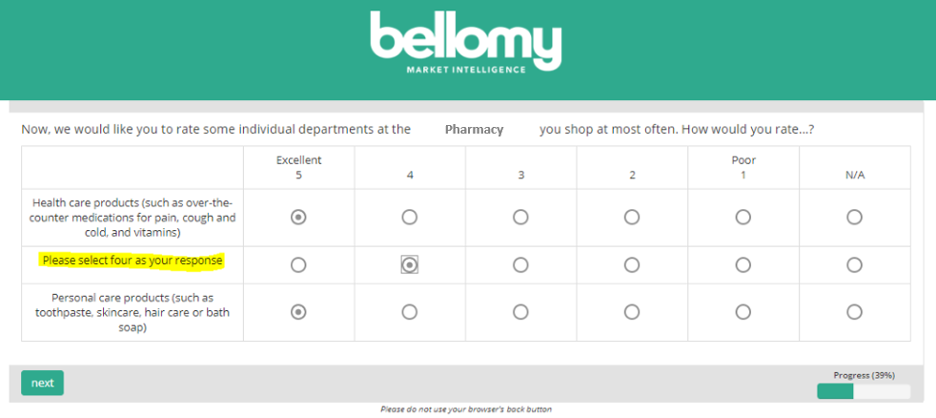
\includegraphics{C:/Users/rees/Documents/R/Projects/LAWYER Hornbooks/5Surveys/SavSurvBlog/SurveyBlog/static/media/BellomyRed.png}
\# shows in script but did not show on the blog via render

If the image isn't generated by R, fig.width and fig.height are
redundant Use PNG for R graphics output, and high-resolution if you plan
to print.

~~~ {[}three \&nbsp{]} indents a paragraph

turn hyperlinks in text into footnotes for PDF output, because readers
will not be able to click the links (generated from \href{URL}{text}).
See
\url{https://bookdown.org/yihui/rmarkdown-cookbook/latex-preamble.html}

blogdown creates a file structure in XX/ that includes these folders:

content (where blog is) layouts (css and js) \#
\url{https://makewithhugo.com/minify-and-load-css-through-hugo/} R
{[}haven't used{]} resources {[}haven't used{]} static (media) .pngs and
other images

Check for bold of key terms, using \textbf{\ldots{}} Insert images with
the Addins drop down Insert URLs as \href{URL}{underlined text} NB no
space \{width=50\%, height=20\%\} didn't work in .md files but does in
.Rmd. Note that there is no space. Opened image in Paint and resized to
70. So I right clicked on the image and chose ``Edit'' and resized. With
the Absinthe painting the original was about 650px by 850. I reduced it
to 60\% and saved, but no difference when I ran the post. No quotes on
file path, no need for directories above BlogThemes1. Underline turns
blue when I do correct syntax.

\begin{verbatim}
Run Check Spelling… in RStudio (under Edit menu)
Run xfun::optipng() on the directory where the post’s images are stored (including plots output by R) for lossless reduction of the size of .png images  [RWM for jpg?]
Run W3C Link Checker on the post preview to make sure all links are valid.
Check images have alt text. A web accessibility evaluation tool can help.  [https://www.w3.org/WAI/ER/tools/]
\end{verbatim}

Save the .md file and check that the changes took (then commit to
GitHub). You can immediately view changes with every save using
LiveReload and your .html file is properly output. Changes are local.
Viewer shows what a user sees on the site.

Save the URL of post on blog by right clicking title and ``Copy link
location''; save the long URL in this file Get the Bitly short form and
add it after the full URL (on Bitly, click ``Create'' orange tab, then
``Link''. Paste in long form and click ``copy'' to save short form; save
below long form)

blogdown::check\_site() will run all check\_*() functions at once.

config.toml has many options, such as changing the name of the site!

\newpage

\hypertarget{creating-a-blog-with-hugo-blogdown-netlify}{%
\section{Creating a blog with Hugo, blogdown,
Netlify}\label{creating-a-blog-with-hugo-blogdown-netlify}}

\hypertarget{changes-to-the-blog-site}{%
\subsection{changes to the blog site}\label{changes-to-the-blog-site}}

Hugo builds the website pages out of blocks of code. If you are using a
straightforward theme like I am then the file at:
/hugo\_root/themes/theme/layouts/\_default/single.html

is the file that builds the pages. This does not contain most of the
HTML that will end up in the final page, rather, it contains calls to
other files that contain the needed HTML. Notably, the header.html and
footer.html files.

If we want to add some custom HTML into the page header then we will
need to add it to the header.html or include a call to another file that
does contain the HTML. We will do that latter as it will be much easier
to keep everything neat if we put the Google Analytics code in its own
file.

useful: rstudioapi::navigateToFile(``config.yaml'') or pick any file

Under /Themes/BlogThemes found config.yaml and changed a number of
features, including title, author, some page names

/BlogThemes/themes/hugo-tanka (changed in early April 2021 to
hugo-texify)

much useful:
\url{https://alison.rbind.io/post/2019-02-19-hugo-archetypes/} also
\url{http://bioinfohippo.rbind.io/tutorials/r_tutorials/2020_05_20_0847-r_blogdown_usefulstuff/}
\url{http://bioinfohippo.rbind.io/tutorials/r_tutorials/2020_05_20_0847-r_blogdown_tutorial/}
\url{http://estebanmoro.org/post/2019-02-02-setting-up-your-blog-with-rstudio-and-blogdown-i-creating-the-blog/}

\url{https://www.r-bloggers.com/2019/01/how-i-started-a-blog-based-on-blogdown-a-walkthrough/}

look in Themes by using Files in Pane 4, and find config. One is
params.toml

When Hugo builds the blog, the final html files and structure go into
the public folder. This is the static version of the blog and the one we
will deploy to our domain.

\hypertarget{learn-about-hugo}{%
\subsubsection{Learn about HUGO}\label{learn-about-hugo}}

\url{https://ropensci.org/blog/2019/01/09/hugo/}

\hypertarget{blog-color-scheme-colorbrewer-palette-dark2httpswww.w3schools.comcsstryit.aspfilenametrycss3_flexbox_justify-content_space-around-try-out-your-code}{%
\subsubsection{Blog color scheme colorBrewer palette
Dark2https://www.w3schools.com/css/tryit.asp?filename=trycss3\_flexbox\_justify-content\_space-around
Try out your
code}\label{blog-color-scheme-colorbrewer-palette-dark2httpswww.w3schools.comcsstryit.aspfilenametrycss3_flexbox_justify-content_space-around-try-out-your-code}}

.customBlogTitle in index.css h1 and header.html navbarLink in
common.css h2 and header.html and header.html, I changed to ``center''
.customPostTitle in index.css h3 subthemes in common.css h4

add extra line To add an extra line of space between paragraphs, add the
HTML ~ code, followed by two extra spaces (e.g.~\&nbsp.., replacing the
periods with spaces).

I used this:
\url{https://colorbrewer2.org/\#type=qualitative\&scheme=Dark2\&n=3}

27,158,119 dark green for Blog Title\\
217,95,2 orangy-red for tabs () 117,112,179 purplish for blog titles\\
subthemes link

\hypertarget{blog-text-font-size-color-and-css-cascading-style-sheets}{%
\subsubsection{Blog text font size, color and css cascading style
sheets}\label{blog-text-font-size-color-and-css-cascading-style-sheets}}

Note: If you do not specify a font size, the default size for normal
text, like paragraphs, is 16px (16px=1em).

BlogTitle Navbar PostTitle

\hypertarget{tabs-at-top-of-blog-navbar-services}{%
\subsubsection{Tabs at top of blog (Navbar):
Services}\label{tabs-at-top-of-blog-navbar-services}}

about.md to modify the About tab.

services.md for my selling pitch

\hypertarget{sidebar-to-list-related-blogs}{%
\section{Sidebar to list related
blogs}\label{sidebar-to-list-related-blogs}}

\url{https://discourse.gohugo.io/t/how-would-i-create-a-sidebar-with-page-specific-related-links/9037/4}

\hypertarget{create-a-form}{%
\subsubsection{create a form}\label{create-a-form}}

I used Formspree to make a contact form, which is an online service
(managed on GitHub) that allows you to add an HTML form to your static
site. No registration, just use the form and confirm your email address
once. I added the following code into my contact widget:
\url{https://alison.rbind.io/post/2017-06-12-up-and-running-with-blogdown/}

\hypertarget{create-box-for-icons}{%
\subsection{Create box for icons}\label{create-box-for-icons}}

config.toml has in it the elements below the blog title, such as About,
Art, Themes, and Subthemes. They have weights that determine their
order.

I created an Icon element to practice boxes and made it weight 5

In BlogThemes1/content I created icon.Rmd

\hypertarget{domain-names-of-savvysurveysjd.com-is-with-namecheap-expires-may-21-2024}{%
\section{domain names of savvysurveysjd.com is with namecheap; expires
May 21,
2024}\label{domain-names-of-savvysurveysjd.com-is-with-namecheap-expires-may-21-2024}}

\hypertarget{one-time-steps-for-gh-netlify-etc.}{%
\subsection{One-time steps for GH, NetLify
etc.}\label{one-time-steps-for-gh-netlify-etc.}}

Later, created GH repository SurveyBlog. Linked it to Render {[}Your
service is always available at \url{https://surveyjds.onrender.com}.{]}.
But in GH, /content/post shows posts in reverse chrono order

\url{https://alison.rbind.io/post/new-year-new-blogdown/} {[}Has three
other posts and is excellent!{]} She wrote the following before:
\url{https://alison.rbind.io/post/2020-12-27-blogdown-checks/}

\begin{verbatim}
I am strongly in favour of never using .Rmd in a blogdown site because its output is an html file, not a .markdown/.md file. from  [RWM but what about inline code?] https://masalmon.eu/2020/02/29/hugo-maintenance/

use .md so Hugo converts to html, but need to edit profile  https://drmowinckels.io/blog/2020-05-25-changing-you-blogdown-workflow/  also need to add archetype to YAML
Third post Alison cites is too complicated https://clauswilke.com/blog/2020/09/08/a-blogdown-post-for-the-ages/
\end{verbatim}

\hypertarget{google-analytics}{%
\subsubsection{Google Analytics}\label{google-analytics}}

\url{https://statsandr.com/blog/track-blog-performance-in-r/} Antoine!

What R package handles Google analytics data? This one lists several
others! do a comparison?
\url{https://code.markedmondson.me/googleAnalyticsR/}

Account Id 188088269 (which is different from the User Authorization
code)

Google Analytics Export Data and Analyze

\hypertarget{analyze-bitly-data-with-r}{%
\subsection{analyze Bitly data with r}\label{analyze-bitly-data-with-r}}

\hypertarget{email-notices-emayili}{%
\section{EMAIL notices emayili}\label{email-notices-emayili}}

\url{https://mvaugoyeau.netlify.app/post/presentation-off-women-international-day/\#sending-the-support-with-the-package-sendmailr}

\url{https://bensstats.wordpress.com/2020/07/23/robservations-2-mail-merging-email-blasting-with-r/}
with emayili

A web browser uses HTTP (Hypertext Transfer Protocol) to communicate
with a web server. Similarly, an email client (like Outlook or
Thunderbird) uses SMTP (Simple Mail Transfer Protocol) as the
communication protocol to send emails.

\hypertarget{sending-message}{%
\subsection{Sending Message}\label{sending-message}}

You can also send an email message directly from a \texttt{mime} object
using \texttt{gm\_send\_message()}.

gm\_auth\_configure() gm\_send\_message(text\_msg)

\hypertarget{six-ways-to-plot-binary}{%
\subsection{Six Ways to plot binary}\label{six-ways-to-plot-binary}}

Adherents of fanplots maintain that they are a better alternative to pie
charts. They represent amounts of values. The traditional pie plot is
difficult for most people to interpret, because humans are not trained
well to observe and interpret angles. This fan plot was generated by the
plotrix package and its fan.plot function.

\end{document}
